\section{Hardware}
In diesem Kapitel wird die Hardware der Steuerung im Detail erläutert. Es wird genauer auf die technischen Details der verwendeten Komponente eingegangen und auf ihre Aufgabe in der Steuerung.

% \begin{itemize}
%     \item Beschreibung, Zweck der TECs
%     \item Beschreibung der TECs und wo diese platziert sind mit Illustrationen
% \end{itemize}

\subsection{Rechner - Raspberry PI}
Abgebildet ist der \textit{Raspberry PI 3B+}. Die SPS, die im nächsten Kapitel beschrieben ist, ist mit dieser Raspberry PI Version kompatibel. Was der Grund ist aus dem der \textit{Raspberry PI 3B+} verwendet wurde.

\begin{figure}
    \centering
    % \includegraphics{}
    \caption{Ein \textit{Raspberry PI 3B+}.}
    \label{fig:raspberry_pi_3b+}
\end{figure}

\subsection{SPS - PiXtend}
Die Aus- und Eingänge, die der Raspberry PI Steuert sind mit einer SPS des Herstellers PiXtend der Version 2.1 realisiert. Dies ist eine Steuerung, auf welche der Rechner direkt aufgeschraubt werden kann. Alle benötigten Ein- und Ausgänge für die Steuerung des Pumpdiodentreibers befinden sich direkt auf der Steuerung. Von grosser Wichtigkeit sind die analogen Ein- und Ausgänge um den Ausgangsstrom des Treibers zu steuern bzw. den Ausgangsstrom zurück in die SPS zu geben, um später die optische Leistung zu evaluieren.

\begin{figure}
    \centering
    % \includegraphics{}
    \caption{Die Energieversorgung}
    \label{fig:sps_pixtend_hw}
\end{figure}

\subsection{Thermoelektrischer Kühler - TEC}
Die beiden verwendeten TECs\footnote{TEC en. Thermo Electric Cooler} werden unter der Pumpdiode bzw. und der Halterung des Alexandritkristalls montiert. Sie dienen dazu die Wärme vom Kristall und von der Pumpdiode ableiten. Werden die Temperaturen an den zu kühlenden bzw. zu heizenden Objekten mit Sensoren gemessen, kann eine optimale Temperatur eingestellt werden.

\begin{figure}
    \centering
    % \includegraphics{}
    \caption{Abgebildet ist ein thermoelektrischer Kühler.}
    \label{fig:tec_free_hw}
\end{figure}

\begin{figure}
    \centering
    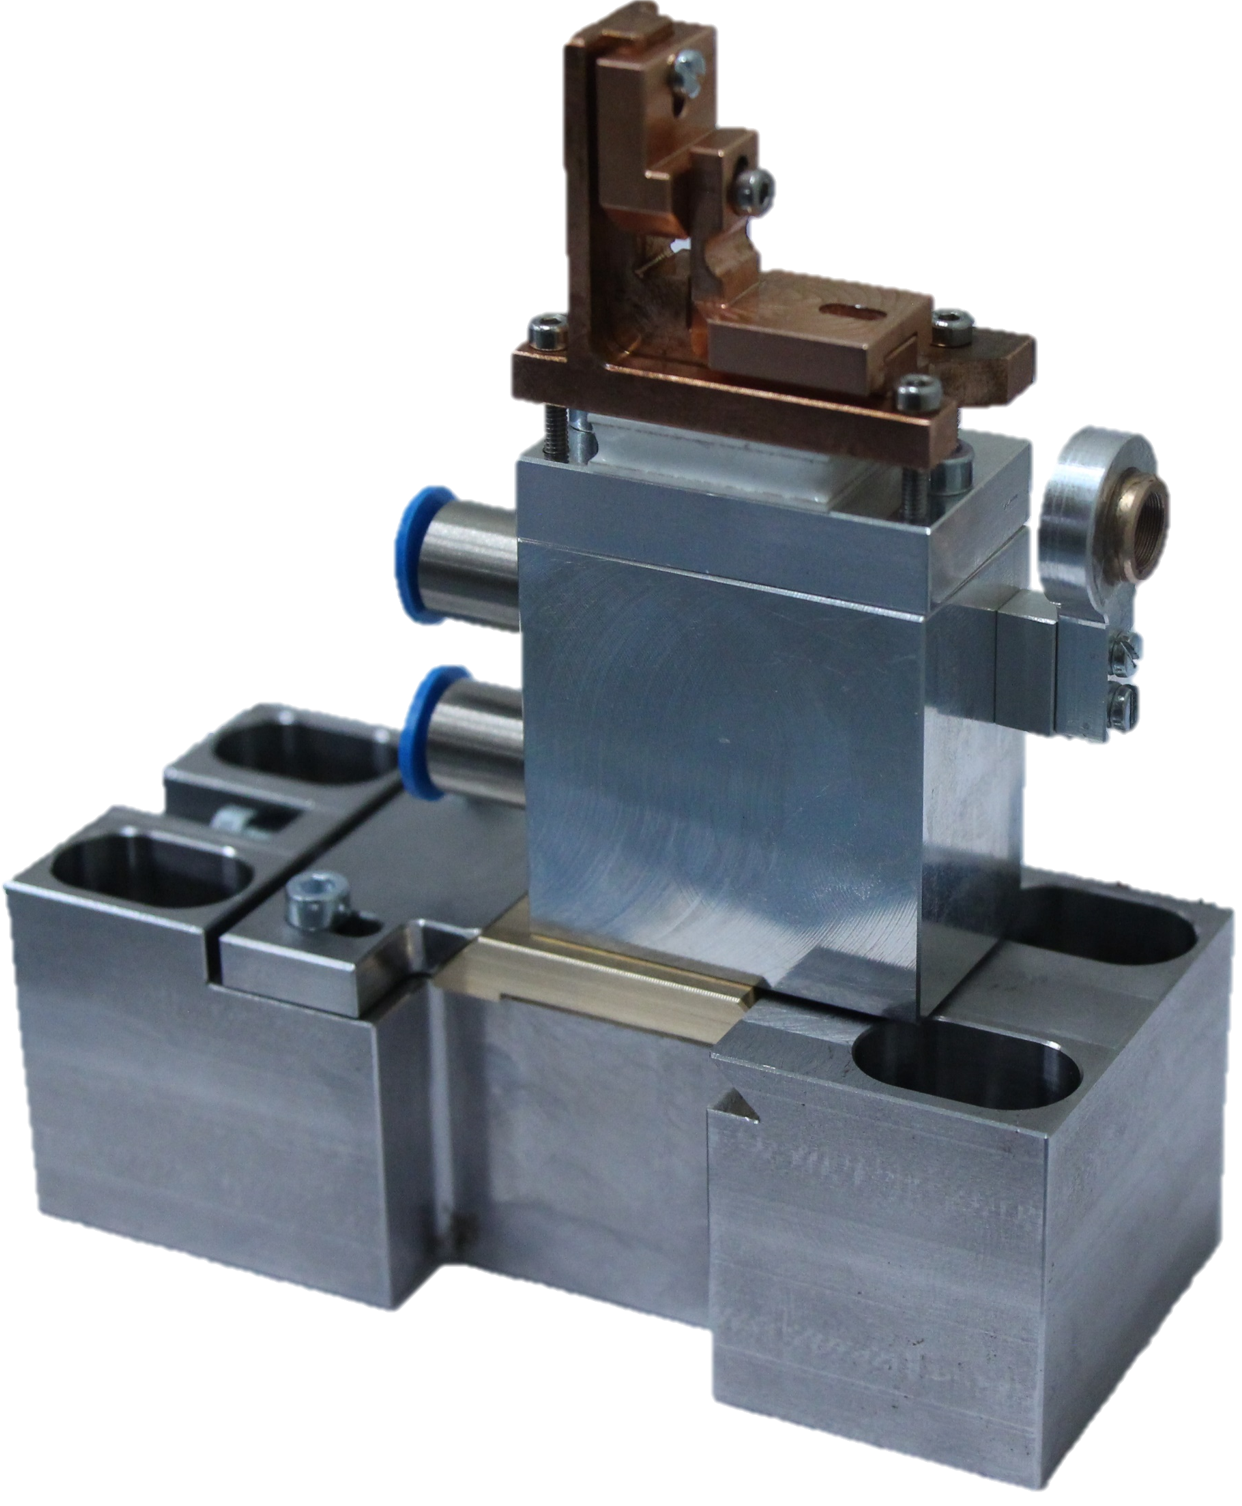
\includegraphics[scale=0.3]{98_images/real_front_02.PNG}
    \caption{In der Abbildung ist der TEC in der Kristallhalterung gezeigt. Dieser befindet sich direkt unter der Halterung des Kristalls. Für den Kristall befindet sich die optimale Temperatur im Bereich von 19°C.}
    \label{fig:tec_cr_hw}
\end{figure}

\begin{figure}
    \centering
    % \includegraphics{}
    \caption{Abgebildet ist der thermoelektrische Kühler für die Diode. Gleich wie beim Alexandritkristall befindet sich dieser direkt unter der Diode. Für eine bessere Wärmeleitung wird einen Wärmeleitpaste auf die Flächen des TECs aufgetragen. Der ideale Temperaturbereich für die Diode ist um die 20°C.}
    \label{fig:tec_di_hw}
\end{figure}

\subsection{TEC-Treiber}
Aus dem Grund, dass zwei TECs gesteuert werden sollen, wurde ein zwei-kanaliger TEC-Treiber des Herstellers Meerstetter Engineering verwendet. Auf der Softwareseite sind die Signale, hier die Temperaturen, eindeutig identifizierbar, was mit zwei einkanaligen Treibern nicht ohne Weiteres möglich gewesen wäre. Die Informationen werden über einen BUS an den Rechner gesendet und da weiter verarbeitet bzw. verwendet.
Die Temperaturen der TECs werden über PID Regler eingestellt. Der Treiber von Meerstetter Engineering ist in der Lage diese PID-Parameter automatisch zu finden und müssen nicht gesucht oder gar berechnet werden. Die TECs können eine maximale Leistung aufnehmen, der Strom muss begrenzt werden, damit sowohl die TECs als auch die Diode oder der Kristall zerstört werden.
% Sicherheit der Diode und der TECs

\begin{figure}
    \centering
    % \includegraphics{}
    \caption{Abgebildet ist der Diodentreiber. Die}
    \label{fig:tec_treiber_hw}
\end{figure}

\subsection{Pumpdiodentreiber}
Der Diodentreiber wurde vom Hersteller \textit{OptLaser} bezogen. Auf der Abbildung sind die Eingänge für die Energieversorgung zu sehen und daneben die analogen bzw. PWM \footnote{PWM:= Puls Weiten Modulation} Eingänge zum steuern des Ausgangstroms.

\begin{figure}
    \centering
    % \includegraphics{}
    \caption{Der Diodentreiber von \textit{OptLaser}}
    \label{fig:diodentreiber_hw}
\end{figure}

\subsection{Energieversorgung}
Die benötigte Leistung des Netzteils für das gesamte System beläuft sich auf etwa 80W.
Dies wurde einerseits errechnet (s. Anhang \ref{formula:_calculation_sp_power}), andererseits mit einem Netzteil an dem alle Komponenten angeschlossen waren verifiziert. Die Pumpdiode wird mit 30V gespiesen, wohingegen der Rest der Steuerung mit 24V betrieben wird. Dies verlangte, das entweder zwei Netzteile eingesetzt werden oder aber ein Netzteil und ein DC/DC-Wandler, der die Spannung des Netzteils auf die benötigten 24V herunter regelt.

\begin{figure}[H]
    \centering
    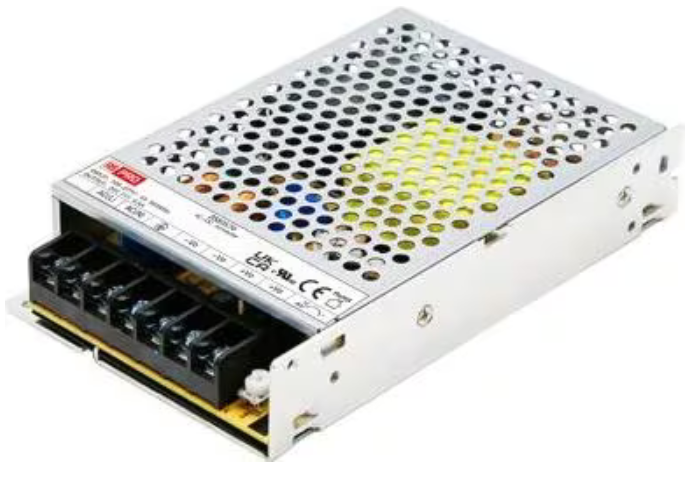
\includegraphics[scale=0.7]{98_images/controller_ps.PNG}
    \caption{Ausgewähltes Netzteil der Marke RS auf Grund der Berechnung 4.1. Es Liefert 24V und 6.5A. Dies entspricht der benötigten Energieversorgung und kann spätere Erweiterungen oder Änderungen aufnehmen.}
    \label{fig:controller_ps_hw}
\end{figure}

\subsection{Sensorik}
Die Positionen der Temperaturmessung des Alexandritkristalls und der Diode sind in Abbildung \ref{fig:temp_measurement_hw} dargestellt. An diesen Positionen stören sie den Laser im Betrieb nicht und können trotzdem die Temperatur möglichst nahe an der Quelle messen.

\begin{figure}
    \centering
    % \includegraphics{}
    \caption{Caption}
    \label{fig:temp_measurement_hw}
\end{figure}

% \subsection{Verkabelung}  % Architektur der Verkabelung
% Die externe Verkabelung des Gehäuses bzw. dessen Komponenten, erfolgt mit einem \textbf{XYZ}-Kabel. Somit können alle Komponente die zum Laser gehen kompakt in einem Kabel geführt werden.\\
% Intern werden die Komponente mit einem \textbf{XYZ}-Kabel verdrahtet und werden über einen Kabelbaum geführt.\textbf{NICHT NÖTIG!!!!!!!!!!}\\

\begin{figure}[H]
    \centering
    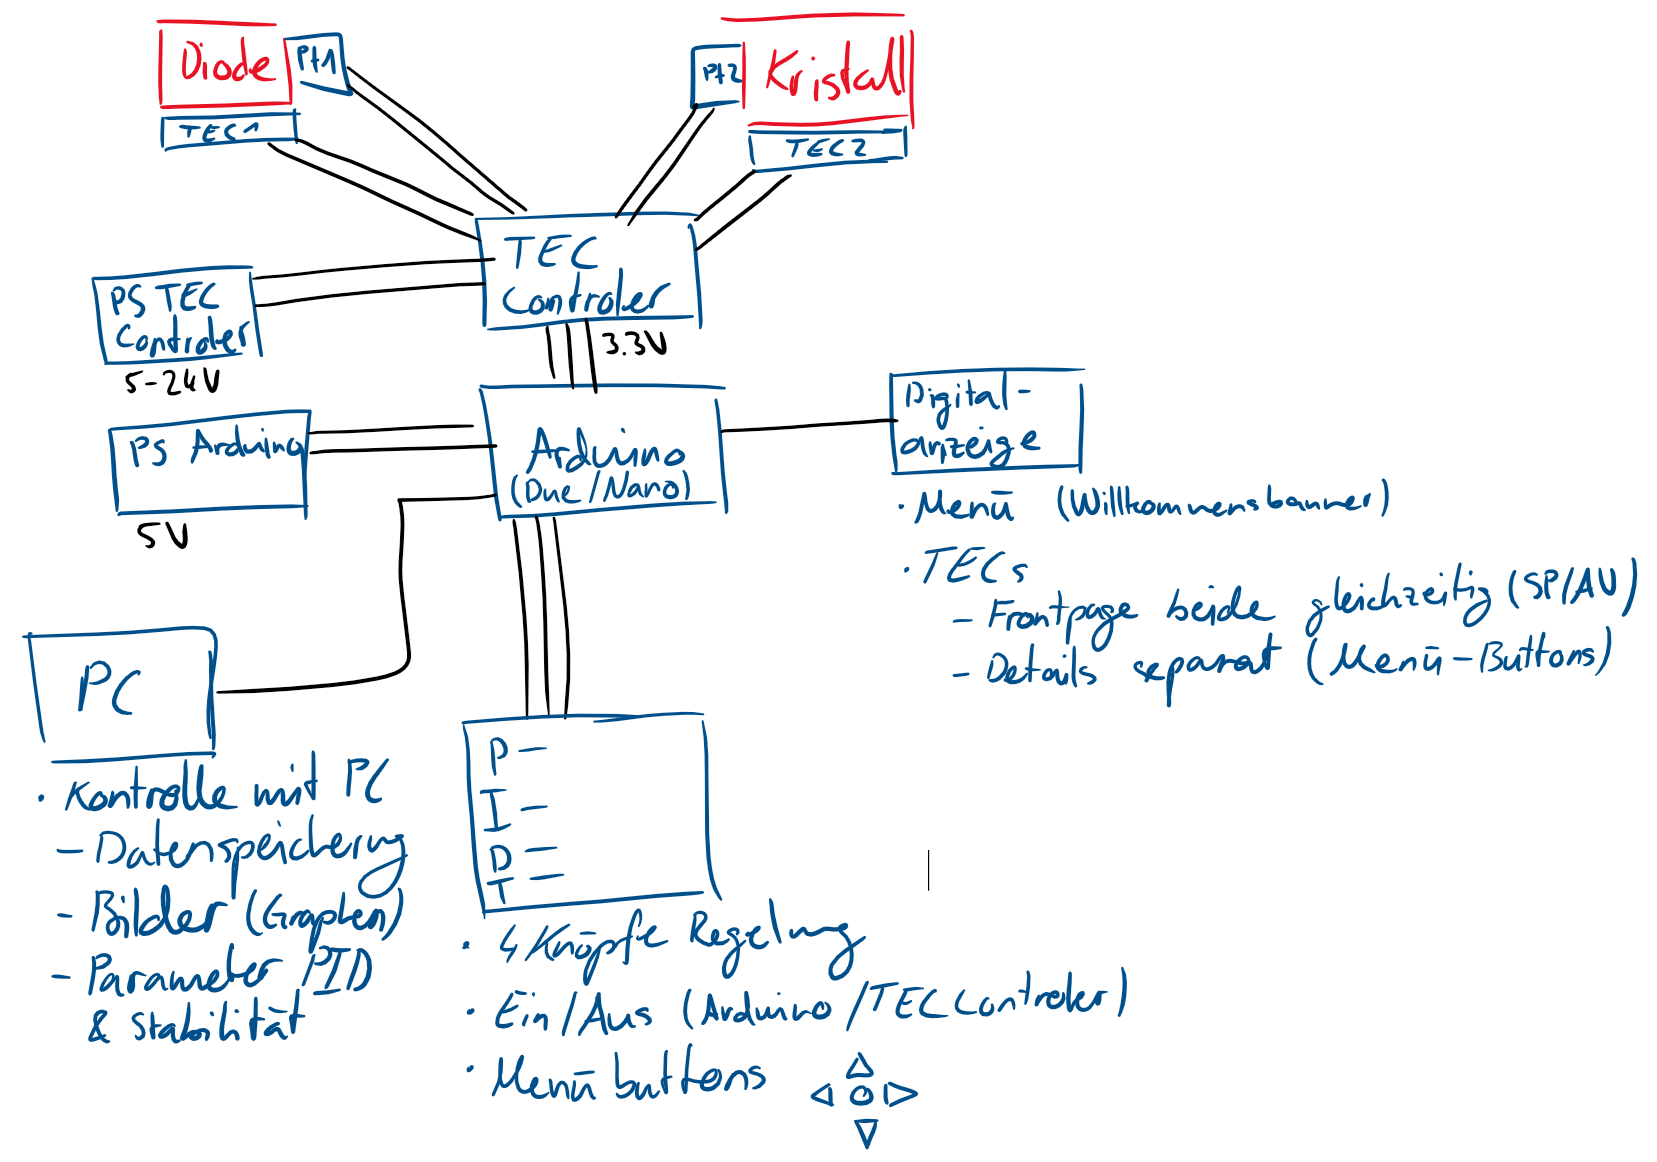
\includegraphics[scale=0.5]{98_images/scheme_wiring.PNG}
    \caption{Verkabelung der elektrischen Komponenten.}
    \label{fig:scheme_wiring_hw}
\end{figure}

\textbf{Auswahl der Digitalanzeige}
Für die Digitalanzeige waren vor allem drei Aspekte ausschlaggebend, um die gewünschte Funktion zu gewährleisten. Die Eingabe der Werte, die Anzeige der Werte und Verständlichkeit der angezeigten Werte. All die Kriterien sollten erfüllt werden, um die Steuerung des Lasers zu gewährleisten. In der Folgenden Tabelle wurden einige Kriterien, die die zuvor genannten Aspekte ermöglichen sollen. Auch aus Sicherheitsgründen muss die Ergonomie der Anzeige intuitiv gestaltet sein und muss im Notfall handhabbar bleiben. Es werden zwei Displaytypen einander gegenüber gestellt.

\begin{table}[H]
    \centering
    \begin{tabular}{l|l}
        \textbf{16x2 mit Taster}&       \textbf{800x400 Touchanzeige}\\
        \hline
        $-$ Taster Analogeingänge&      $+$ Integriert\\
        $-$ Kleine Anzeige&             $+$ Grössere Anzeige\\
        $-$ Kryptische Anzeige&         $+$ Verständliche Anzeige\\
        $-$ Tieferes Menü&              $+$ Weniger tiefes Menü\\
        $+$ Einfache Programmierung&    $-$ Anspruchsvolle Programmierung\\
    \end{tabular}
    \caption{Pro - Kontra Liste für die Auswahl der Digitalanzeige}
    \label{tab:choice_display_hw}
\end{table}

Die Entscheidung fiel auf die Touchanzeige. Zusätzlich lassen sich alle Komponente wie Knöpfe direkt in die Anzeige programmieren. Es müssen keine komplexen Abläufe programmiert werden, die die Betätigung der physischen Knöpfe erkennt und das Programm lenkt. Zusätzlich müssen keine Ein-/Ausgänge zusätzlich auf der SPS einprogrammiert werden. Mit der Anzeige können ganze Designs erstellt werden, was das Arbeiten mit der Steuerung ergonomischer macht.

\subsection{Konstruktion des Gehäuses}
Das Gehäuse war bereits vorhanden. Die oben aufgelisteten Komponenten wurden auf zusätzlichen Blechen montiert, in die Gewindelöcher eingebracht wurden. Durch die konvexe Form der Seiten des Gehäuses entstand im Inneren des Kontrollers mehr Fläche für die Komponenten und vereinfachte dadurch die Montage. Zusätzlich mussten noch die Zugänge für die Verkabelung der Stromversorgung, deren Schalter und das Kabel für die Ansteuerung der Komponenten im Laser-Aufbau angepasst werden. Dafür wurden sämtliche Löcher für spätere Erweiterungen beibehalten.

\subsection{Testaufbau - Mock-up}
In einem Mock-up konnten die Funktionen und das Verhalten der Steuerung geprüft werden. Darunter wurde getestet, ob die Temperaturen in der Steuerung in einem gewünschten Rahmen von 40°C-65°C blieben. $[13]$ Zur Referenz wurde die interne Messung der CPU verwendet. Gemessen werden die Temperaturen mit der internen Temperaturmessung des Prozessors des Raspberry PI. Die Temperatur im Gehäuse wurde dann von der Temperatur des Prozessors abgeleitet. Dafür wurde sie mit einem Temperaturmessgerät extern gemessen und die Messergebnisse mit denen des Prozessors verknüpft.
Die Positionen der Komponenten im Gehäuse wurde mit Hilfe von CAD-Software geprüft. Dafür wurden die oben genannten Bleche erstellt und die Komponente mit Verschraubungen platziert.